\chapter{Allgemeines}
		\section{Arten von Sicherheit}
			Grundlegend wird zwischen Betriebssicherheit (engl. \textit{safety}) und Angriffssicherheit (engl. \textit{security}) unterschieden.\\
			\textbf{Angriffssicherheit} ist der Schutz vor aktiven Angreifern mit Schadabsicht.\\
			\textbf{Betriebssyicherheit} ist der Schutz vor Fehlern innerhalb des Systems, das Sichern der Zuverlässigkeit und der Schutz vor äußeren Faktoren wie Umwelteinflüssen.
			
		\section{Schutzziele der Angriffssicherheit}
			Man versucht die folgenden Schutzziele zu erreichen:
			\begin{itemize}
				\item \textbf{Authentizität}: Die empfangenen Daten stammen von dem Absender, mit dem man kommunizieren möchte.
				\item \textbf{Integrität}: Die Daten wurden auf dem Weg nicht verändert und stammen genau so vom Absender.
				\item \textbf{Vertraulichkeit}: Die Daten können auf dem Kommunikationsweg nicht von anderen gelesen werden.
				\item \textbf{Nicht-Abstreitbarkeit}: Dem Absender kann nachgewiesen werden, dass er die Daten verschickt hat.
				\item \textbf{Verfügbarkeit}: Das System soll jederzeit verfügbar sein und vor Ausfall geschützt sein.
			\end{itemize}
			
		\section{Schutzziele der Betriebssicherheit}
			Man versucht die folgenden Schutzziele zu erreichen:
			\begin{itemize}
				\item \textbf{Schutz vor Ausfall}: bespielsweise soll ein Signal bei Stromausfall nach unten klappen und damit „Halt“ (Hp 0) zeigen, um größere Schäden zu verhindern.
				\item \textbf{Redundanz}: Kritische Systeme sollten bei Ausfall durch Backupsysteme ersetzt werden können. Daten sollten gesichert sein.
				\item \textbf{Schutz vor Architektur-/Softwarefehlern}: beispielsweise sollten Overflows von Variablen verhindert werden.
			\end{itemize}
			
		\section{Angriffe}
			Die meisten Angriffe haben finanzielle Interessen. Nutzerdaten und Gelder lassen sich digital übernehmen und sind wertvoll.\\
			Mögliche Angriffe sind:
			\begin{itemize}
				\item \textbf{Phishing}: Ausliefern einer ähnlich aussehenden, gefälschten Website, damit Nutzer ihre Zugangsdaten eingeben.
				\item \textbf{Man-in-the-Middle}: Abgreifen von Daten, indem man sich in die Mitte der Verschlüsselungsverbindung stellt und mit jedem Partner einzeln verschlüsselt (und vortäuscht, der jeweils andere zu sein).
			\end{itemize}
			
			
\chapter{Kryptographie}
	Durch Kryptographie können die oben genannten Schutzziele erreicht werden.\\Außerdem ist die Kryptoanalyse, also das Nachweisen der Sicherheit und Angreifen auf Kryptographieverfahren, in diesem Fall Teil der Kryptographie.
	
	\section{Begriffe}
	\begin{itemize}
		\item \textbf{Klartext}: die unverschlüsselte Nachricht
		\item \textbf{Klartextraum}: die Menge aller möglichen Klartexte
		\item \textbf{Chiffrat}: die verschlüsselte Nachricht
		\item \textbf{Chiffratraum}: die Menge aller möglichen verschlüsselten Nachrichten
		\item \textbf{Verschlüsselung}: der Vorgang der Umwandlung eines Klartexts in ein Chiffrat
		\item \textbf{Entschlüsselung}: der Vorgang der Umwandlung eines Chiffrats in einen Klartext
		\item \textbf{Schlüssel}: ein Geheimnis, das benötigt wird, um eine Nachricht ver-/entschlüsseln zu können
		\item \textbf{Schlüsselraum}: die Menge aller möglichen Schlüssel
		\item \textbf{Kryptosystem}: eine Ver-/Entschlüsselungsvorschrift mit zugehörigem Klartextraum, Chiffratraum und Schlüsselraum
	\end{itemize}
	
	\section{Mathematische Grundlagen}
	Die hier nicht weiter beschriebenen mathematischen Grundlagen sind wie in der Mathematik üblich definiert.
	
		\subsection{Euklidischer Algortithmus}
		\underline{Einfacher euklidischer Algorithmus:}\\\\
		Seien $a\neq0, b\in\mathbb{Z}$.\\ Dann liefert der folgende Algorithmus den größten gemeinsamen Teiler von a und b:
		\begin{lstlisting}
a = |a|; b = |b|;
while (b > 0):
	if (a > b):
		a = a - b;  | Alternativ: a = a mod b;
	else:
		b = b - a;  | Alternativ: b = b mod a;
return a;
		\end{lstlisting}
		
		\newpage
		
		\underline{Erweiterter euklidischer Algorithmus:}\\\\
		Seien $a,b\neq0\in\mathbb{Z}$.\\ Dann liefert der folgende Algorithmus den größten gemeinsamen Teiler von a und b:
		\begin{lstlisting}
a_0 = max(|a|, |b|); b_0 = min(|a|, |b|); n = 0;
while (b_n > 0):
	q_n = (int) a_n / b_n;
	r_n = a_n / b_n - q_n; // a_n mod b_n
	a_{n+1} = b_n; b_{n+1} = r_n;
	n = n + 1;
return a;
		\end{lstlisting}
		Nun gilt:\\
		$ggT(a,b) = a_n = b_{n-1} = r_{n-2} = a_{n-2} - q_{n-2}b_{n-2} = b_{n-3} - q_{n-2}r_{n-3}=...=x\cdot a_0+y\cdot b_0= ax+by$\\
		
		\begin{multicols}{3}
		[Der EEK lässt sich auch in Tabellenform lösen:\\
		(a, b, q intuitiv nach unten; dann von unten $s=t_{alt}$, $t=s_{alt}-q\cdot t_{alt}$)]
		
		\begin{tabular}{|c|c|c|c|c|}
		\hline
		a & b & q & s & t\\ \hline
		99 & 78 & 1 & -11 & 14 \\
		78 & 21 & 3 & 3 & -11 \\
		21 & 15 & 1 & -2 & 3 \\
		15 & 6 & 2 & 1 & -2 \\
		6 & 3 & 2 & 0 & 1 \\
		3 & 0 & & 1 & 0 \\\hline		
		\end{tabular}

		\columnbreak\columnbreak			
		
		\begin{tabular}{|c|c|c|c|c|}
		\hline
		a & b & q & s & t\\ \hline
		61 & 13 & 4 & 3 & -14 \\
		13 & 9 & 1 & -2 & 3 \\
		9 & 4 & 2 & 1 & -2 \\
		4 & 1 & 4 & 0 & 1 \\
		1 & 0 & & 1 & 0 \\\hline		
		\end{tabular}			
		\end{multicols}		
		$ $\\$99\cdot (-11)+78\cdot 14=-1089+1092=3$\\$61\cdot3+13\cdot(-14)=183-182=1$
		
		\subsection{Lemma von Bézout}
		$\forall a,b\in\mathbb{Z}: \exists x,y\in\mathbb{Z}: ax+by=ggT(a,b)$
		
		\subsection{Eulersche Phi-Funktion}
		$\varphi(b):=|\{a\in\mathbb{N} | a < b, ggT(a,b) = 1\}|$\\\\
		Es gilt (p prim):\\
		$\varphi(p)=p-1$\\
		$\varphi(p^n)=p^n-p^{n-1}$\\
		$\varphi(ab)=\varphi(a)\cdot\varphi(b)$\\\\
		
		\underline{Euler-Fermat:}\\
		$\forall m,n\in\mathbb{N}: \textbf{m,n teilerfremd} \Rightarrow m^{\varphi(n)} mod n = 1$
		
	\newpage

	\section{Kerckhoffs Prinzipien}
	Diese Prinzipien sollte jedes Kryptosystem erfüllen.
	\begin{enumerate}
		\item Das System ist zumindest praktisch unknackbar. Ohne Kenntnis des Schlüssels ist der Klartext nicht innerhalb eines praktikablen Zeitraums errechenbar. Optimalerweise ist die Sicherheit mathematisch beweisbar.
		\item Die Geheimhaltung des Verfahrens ist für die Sicherheit nicht erforderlich. Das gemeinsame Kennen eines Geheimnisses (Schlüssel) reicht aus, um Sicherheit zu garantieren.\\ \textit{In der Vergangenheit hat sich gezeigt, dass öffentliche Verfahren, bei denen jeder die Sicherheit prüfen kann, zu mehr Sicherheit führen als geheimgehaltene Verfahren.}
		\item Der Schlüssel muss ohne Hilfe geschriebener Notizen kommunizierbar und aufbewahrbar sein und muss  nach Belieben der
Kommunikationspartner ausgewechselt oder modifiziert werden können.\\ \textit{Dieses Ziel ist heute nicht mehr umsetzbar und wird weitgehend nicht mehr beachtet.}
		 \item Es muss auf telegraphische Kommunikation anwendbar sein.
		 \item Es soll portabel sein und nicht voraussetzen, dass sich mehrere Menschen treffen.
		 \item Es muss einfach von jedem anwendbar sein.
	\end{enumerate}
	
	\section{Angriffe}
	Diesen Angriffsszenarien sollte eine sichere Verschlüsselung standhalten können:
	\begin{enumerate}
		\item \textbf{known chiffretext}: Der Angreifende kennt den verschlüsselten Text (Chiffrat)
		\item \textbf{known plaintext}: Der Angreifende kennt den verschlüsselten Text (Chiffrat) und den Klartext einer alten Nachricht und versucht nun mithilfe des Chiffrats einer neuen Nachricht, diese zu entschlüsseln.
		\item \textbf{chosen plaintext}: Der Angreifer kann Chiffrate zu beliebigen Klartextnachrichten mithilfe des Verfahrens generieren.
		\item \textbf{chosen chiffretext}: Der Angreifer kann Klartexte zu beliebigen Chiffraten mithilfe des Verfahrens generieren.
	\end{enumerate}
	
	\section{Symmetrische Kryptosysteme}
	Symmetrische Verschlüsselungsverfahren sind daran erkennbar, dass es eine Verschlüsselungsfunktion $e:\mathcal{M}\times\mathcal{K}\rightarrow\mathcal{C}$ und eine Entschlüsselungsfunktion $d:\mathcal{C}\times\mathcal{K}\rightarrow\mathcal{M}$ gibt.
	
		\subsection{Verschiebechiffre (Cäsar, ROT13)}
			Sei $z$ die Menge der im Klartext zugelassenen Zeichen und $|z|=n\in\mathbb{N}$. Nun lege man eine Bijektion $f$ zwischen den Zeichen und $[0;n-1]\in\mathbb{N}$ fest. Dann berechne man für den Klartext $z^x$ für jedes einzelne $z$ das verschlüsselte Zeichen $e:=f^{-1}(f(z) + s \text{ (mod $n$)})$ für einen gegebenen Schlüssel $s\in [0;n-1]\in\mathbb{N}$. Dann ist $z=f^{-1}(f(e)-s \textbf{ (mod $n$)})$.\\
			Das Verfahren ist jedoch nicht sicher, da die Schlüsselmenge zu gering ist, Häufigkeitsanalyse möglich ist und merere weitere Angriffsverfahren (s. oben) funktionieren.
			
		\subsection{Vignière-Chiffre}
			Die Vignière-Chiffre ist im Prinzip eine Verschiebechiffre mit verschiedenem Schlüssel für jeden Buchstaben. Damit der Schlüssel kürzer als die Nachricht ist, wiederholt man diesen jedoch alle paar Zeichen, wodurch eine Häufigkeitsanalyse zwar schwerer aber noch möglich ist.
		\subsection{One-Time-Pad}
			Bei einem One-Time-Pad hat der Schlüssel die gleiche Länge wie die Nachricht (jeweils in Binärdarstellung). Nun berechnet man die n-te Stelle der verschlüsselten Nachricht meist durch Anwenden von XOR auf die n-te Stelle der Eingabe und der n-ten Stelle des Schlüssels. Dieses Verfahren ist kryptographisch sicher. Der Klartext lässt sich auf die gleiche Weise mit dem Schlüssel wieder berechnen.
			
		\subsection{Blockchiffre}
			\subsubsection{ECB: Electronic Codebook}
			Der Klartext wird in Blöcke fester Länge zerlegt und auf jeden einzelnen Block wird eine Verschlüsselungsfunktion (z. B. ein One-Time-Pad) mit gleichem Schlüssel angewendet. Nötigenfalls wird die Klartextnachricht vorher mit Binärwerten aufgefüllt. Dieses Verfahren ist offensichtlich nicht sicher (s. verschlüsseltes TU Darmstadt-Logo in den Vorlesungsfolien).
			
			\subsubsection{CBC: Cipher Block Chaining}
			Vor der Verschlüsselung des ersten Blocks wird hier noch ein (nicht geheimer) Schlüssel aus Zufalsswerten (sog. Initialisierungsvektor) addiert (XOR) und anschließend dieser Teil verschlüsselt. Der verschlüsselte Teil dient nun als IV für den nächsten Block usw.\\Wenn jeder Schlüssel nur bei einer Verschlüsselung eingesetzt wird, ist dieses Verfahren sicher.\\
			Zur Entschlüsselung wird jeder Ciphertext erst entschlüsselt und anschließend der Ciphertext des vorhergehenden Blocks addiert (XOR) (beim ersten Block wird der IV verwendet). Dadurch ist die Entschlüsselung im Gegensatz zur Verschlüsselung parallelisierbar.
			
			\subsubsection{CTR/CTM: Counter Mode}
			Im CTR Mode wird erst die Verschlüsselung auf das Resultat einer Operation auf einer Nonce und einem mit jedem Block inkrementierten Counter angewendet. Anschließend wird diese auf den Klartext addiert (XOR). Die Entschlüsselung funktioniert entsprechend.\\
			Dieser Modus ist eine Stromchiffre.
		
		
	\section{Asymmetrische Kryptosysteme}
		Bei asymmetrischen Verschlüsselungsverfahren hat jeder einen privaten und einen öffentlichen Schlüssel. Mithilfe des öffentlischen Schlüssels können Nachrichten an die Person verschlüsselt werden. Mithilfe des privaten Schlüssels können sie wieder entschlüsselt werden.
		
		\subsection{RSA}
		\underline{Schlüsselgenerierung:}
		\begin{enumerate}
			\item Wähle Primzahlen $p$ und $q$.
			\item Berechne $n=p\cdot q$ und $\varphi(n)=(p-1)\cdot(q-1)$.
			\item Wähle $e$ mit $e<\varphi(n)$ und $\text{ggT}(e,\varphi(n))=1$.
			\item Wähle $d$ mit $d<\varphi(n)$ und $e\cdot d\mod\varphi(n)=1$.
		\end{enumerate}
		\underline{Ver-/Entschlüsselung:}
		\begin{itemize}
			\item Verschlüsselung: $c=m^e\mod n$
			\item Entschlüsselung: $m=c^d\mod n$
		\end{itemize}
		
		\subsection{ElGamal}
		\underline{Schlüsselgenerierung:}
		\begin{itemize}
			\item Wähle zyklische Gruppe $\mathcal{G}=(G,\circ,e)$ und $g,a\in\{2,...,ord(G)-1)$. Berechne nun $A=g^a$.
			\item Dann ist der private Schlüssel $(\mathcal{G},g,a)$.
			\item Dann ist der öffentliche Schlüssel $(\mathcal{G},g,A)$.
		\end{itemize}
		\underline{Verschlüsselung:}
		\begin{enumerate}
			\item Wähle $r\in\{2,...,ord(G)-1)$ und berechne $R=g^r$.
			\item Berechne $K = A^r = (g^a)^r$ und $C = m\circ K$.
			\item Übermittle $C$ und $R$.
		\end{enumerate}
		\underline{Entschlüsselung:}
		\begin{enumerate}
			\item Berechne $K = R^a = (g^r)^a = (g^a)^r$ und $C = m\circ K$.
			\item Berechne $K^{-1}$ in $\mathcal{G}$.
			\item Berechne $C\circ K^{-1} = m\circ K\circ K^{-1} = m$.
		\end{enumerate}
		
	\section{Hybride Verschlüsselung}
		Bei Hybrider Verschlüsselung wird der Schlüssel für die symmetrische Verschlüsselung mit asymmetrischer Verschlüsselung verschlüsselt, wodurch die langsamere, asymmetrische verschlüsselung weniger verschlüsseln muss. Die Sicherheit ist dadurch aber von beiden Kryptosystemen abhängig.
		
	\section{Hash und Signatur}
		\subsection{Definition}
		Eine \textbf{Hashfunktion} ist für $n\in\mathbb{N}$ eine Funktion $h:A^*\rightarrow A^n$.\\
		Eine \textbf{Kompressionsfunktion} ist für $m,n\in\mathbb{N},n<m$ eine Funktion $h:A^m\rightarrow A^n$.\\\\
		Es geht jeweils darum Nicht-Abstreitbarkeit, Authentizität und Integrität zu garantieren.
		
		\subsection{Kollisionsresistenz}
		Eine Funktion heißt \textbf{schwach kollisionsresistent}, wenn es zu gegebenem $x_1$ schwer ist, ein $x_2$ zu finden mit $h(x_1)=h(x_2)$.\\
		Eine Funktion heißt \textbf{stark kollisionsresistent}, wenn es schwer ist, $x_1$ und $x_2$ zu finden mit $h(x_1)=h(x_2)$.
		
		\subsection{Merkle-Darmgård}
		Mithilfe dieser Konstruktion lässt sich aus einer Kompressionsfunktion eine Hashfunktion kreieren:\\
		Sei $A$ ein Alphabet und $f:A^{n+m}\rightarrow A^n$ eine Kompressionsfunktion.\\
		Sei $pad:A^*\rightarrow (A^m)^*$ eine Auffüllfunktion.\\
		Sei $h_0\in A^n$ ein beliebiger Initialisierungsvektor und $g:A^n\rightarrow A^n$ eine Finalisierungsfunktion.\\
		Dann sei $h:A^*\rightarrow A^n$ für $x\in A^*$ wie folgt zu berechnen:
		\begin{enumerate}
			\item $x_1\cdot x_2\cdot...\cdot x_k=pad(x)$ mit $x_i\in A^m$ für $i\in[1,k]\subset\mathbb{N}$.
			\item $h_i=f(append(h_{i-1},x_i))$ für $1\leq i\leq k$.
			\item $h(x) = g(h_k)$.
		\end{enumerate}
		
		\subsection{RSA-Signatur}
		Wendet man auf eine Nachricht $m$ eine Hashfunkion $h$ mit Zielbereich zwischen $0$ und $n$ an, so erhält man durch $s=h(m)^d\mod n$ die Signatur. Mit dem öffentlichen Schlüssel kann dann jeder prüfen, ob die Signatur korrekt ist, denn dies ist genau dann der Fall, wenn $h(m)=s^e\mod n$.\\ Das Hashen ist hier unbedingt erforderlich, da man sonst aus $(m,s)$ eine neue signierte Nachricht $(s^e,s)$ generieren könnte, ohne den privaten Schlüssel zu kennen.
		
		\subsection{DSA: Digital Signature Algorithm}
		\underline{Parametergenerierung}
		\begin{enumerate}
			\item Wähle Primzahl $q$ und sehr große Primzahl $p$ mit $q\mid (p-1)$.
			\item Für ein $1<h<p-1$, berechne $g=h^\frac{p-1}{q}$. Es ist also $ord(g)=q$.
			\item $p$, $q$ und $g$ können öffentlich sein und von mehrere Nutzern verwendet werden.
		\end{enumerate}
		\underline{Schlüsselgenerierung}
		\begin{enumerate}
			\item Wähle $x$ mit $1<x<q$ zufällig.
			\item Berechne $y=g^x\mod p$.
			\item $y$ ist der öffentliche Schlüssel, $x$ ist der private Schlüssel.
		\end{enumerate}
		\underline{Signieren}
		\begin{enumerate}
			\item Wähle $k$ mit $1<k<q$.
			\item Berechne $r = max((g^k\mod p)\mod q,1)$.
			\item Berechne $s = max(k^{-1}\cdot(H(m)+r\cdot x)\mod q,1)$.
			\item Sie Signatur ist nun das Tupel $(r,s)$.
		\end{enumerate}
		\underline{Verifikation}
		\begin{enumerate}
			\item Berechne $w=s^{-1}\mod q$.
			\item Berechne $u_1=H(m)\cdot w\mod q$.
			\item Berechne $u_2=r\cdot w\mod q$.
			\item Berechne $v=(g^{u_1}\cdot y^{u_2}\mod p)\mod q$.
			\item Akzeptiere wenn $v=r$.
		\end{enumerate}
		
	\section{Schlüsselaustausch/-generierung}
		\subsection{Needham-Schroeder (symmetrisch)}
		Annahme: Alle haben mit T einen Schlüssel ausgetauscht. A und B wollen kommunizieren. $N_A$ und $N_B$ sind Nonce.
		\begin{enumerate}
			\item $A\rightarrow T$: $A,B,N_A$
			\item $T\rightarrow A$: $\{N_A,K,B,\{K,A\}_{K_B}\}_{K_A}$
			\item $A\rightarrow B$: $\{K,A\}_{K_B}$
			\item $B\rightarrow A$: $\{N_B\}_K$
			\item $A\rightarrow B$: $\{N_B-1\}_K$
		\end{enumerate}
		Wenn ein Angreifer einen alten Schlüssel hat, kann er allerdings mit B eine Verbindung aufbauen und sich als A ausgeben. Dies kann durch einen Zeitstempel verhindert werden.
		
		\subsection{Needham-Schroeder (asymmetrisch)}
		Es gibt auch eine asymmetrische Variante ($K_{P_A}$ und $K_{P_B}$ sind öffentliche Schlüssel, $K_{S_T}$ ist ein privater Signaturschlüssel):
		\begin{enumerate}
			\item $A\rightarrow T$: $A,B$
			\item $T\rightarrow A$: $\{K_{P_B},B\}_{K_{S_T}}$
			\item $A\rightarrow B$: $\{N_A,A\}_{K_{P_B}}$
			\item $B\rightarrow T$: $B,A$
			\item $T\rightarrow B$: $\{K_{P_A},A\}_{K_{S_T}}$
			\item $B\rightarrow A$: $\{N_A,N_B\}_{K_{P_A}}$
			\item $A\rightarrow B$: $\{N_B\}_{K_{P_B}}$
		\end{enumerate}
		Wenn ein Angreifer einen alten Schlüssel hat, kann er allerdings mit B eine Verbindung aufbauen und sich als A ausgeben. Dies kann durch einen Zeitstempel verhindert werden.
		
		\subsection{Diffie-Hellmann}
		\underline{Funktionsweise:}
		\begin{enumerate}
			\item Wähle zyklische Gruppe $\mathcal{G}$ der Ordnung $p$ (prim) und einen Generator $g\in\mathcal{G}$.
			\item $A$ wählt $0<a<p$ und berechnet $g^a$. $B$ wählt $0<b<p$ und berechnet $g^b$.
			\item $g^a$ und $g^b$ werden ausgetauscht.
			\item Beide können nun $g^{ab}$ berechnen.
		\end{enumerate}
		Allerdings sind Vorberechnungen bei bekannter zyklischer Gruppe für selbige möglich.\\
		Um MitM-Angriffe zu verhindern, sollten die Nachrichten signiert werden (Station-to-Station).
		
		\section{AE(AD): Authenticated Encryption (with Associated Data)}
		\underline{AE:} Daten sollen verschlüsselt und unmanipulierbar sein.\\
		Es gibt verschiedene Möglichkeiten:
		\begin{enumerate}
			\item EtM (Encrypt-then-MAC): [Bsp.: IPSec] Nachricht wird verschlüsselt. Anschließend wird dies und der Hash davon übertragen.
			 \item MtE (MAC-then-Encrypt): [Bsp.: TLS] Nachricht und deren Hash werden zusammen verschlüsselt.
			\item E\&M (Encrypt-and-MAC): [Bsp.: SSH] Nachricht wird verschlüsselt und Hash der Nachricht angefügt.
		\end{enumerate}
		%\todo{Galois Counter Mode 7}
		\underline{AEAD:} Unverschlüsselte Metadaten sollen zusätzlich übertragen werden. Die Integrität soll weiterhin gewährleistet sein.
		
		\section{Secret Sharing}
		Daten sollen nur entschlüsselt werden können, wenn $t$ von $n$ Beteiligten mitwirken.\\
		Möglichkeit: $\binom{n}{t}$ verschiedene Verschlüsselungen
		
		\subsection{Shamirs Secret Sharing Protokoll}
		Sei $k$ der Schlüssel. Es gebe $n$ Shareholder mit Thresholt $t$.\\
		Es wird zentral vom \textit{Dealer} eine Primzahl $p$ mit $p>k$ und $p>n$ gewählt. Wir rechnen nun in $\mathbb{Z}_p$.\\
		Der Dealer wählt ein Polynom $\sum\limits_{i=0}^{t-1}f_i\cdot x^i$ mit $f(0)=k$.\\Nun verteilt der Dealer $\{s_1,s_2,...,s_n\}=\{(1,f(1)),(2,f(2)),...,(n,f(n))\}$ an die einzelnen Beteiligten.
		%\todo{Rückschluss}
		
	
		
\chapter{IT-Sicherheit und Zuverlässigkeit}

	\section{Zugriffsrechte}
	
		\subsection{DAC: Discretionary Access Control}
		Hier ist der Eigentümer für die Rechtevergabe verantwortlich. Für jede Kombination aus Zugreifendem und Datei können alle Rechte explizit gesetzt werden. Rechteänderungen sind allerdings schwer umzusetzen und nur Schreibzugriff auf das eigene Passwort in der Passwortdatei zu gewähren ist schwer. Statt einer Zugriffsmatrix (Datei $\leftrightarrow$ Prozess) kann auch eine Access Control List (ACL) eingesetzt werden, damit Rechte an einer Datei effizient bestimmbar sind. Bei dynamischen Subjektmengen ist dies allerdings schlecht skalierbar.\\In Unix-Systemen werden die Rechte read, write und execute für Besitzer, Gruppe und Andere gespeichert.\\Auch eine subjektbezogene Rechtespeicherung ist denkbar, allerdings weitgehend nicht praktikabel.
		
		\subsection{RBAC: Role-based Access Control}
		Es wird eine Zuordnung von Subjekten auf Gruppenzugehörigkeit zu allen existierenden Gruppen gespeichert und eine Rechtezuordnung von jeder Gruppe zu möglichen Rechten.\\In dieser Modellierung können Rechte mithilfe einer partiellen Ordnung (antisymmetrisch, reflexiv, transitiv) auf den Gruppen auch vererbt werden.
		
		\subsection{MAC: Mandatory Access Control}
		Subjekte und Objekte bekommen jeweils Sicherheitsstufen zugewiesen. Danach wird entschieden, auf welche Dateien wer zugreifen darf. Es existiert eine Zuordnung zwischen den Gruppen der Subjekte und den Sicherheitsstufen der Objekte.
	%\todo{Vor-/Nachteile}
	
	\section{Authentifizierung}
	
		\subsection{Begriffe}
		\begin{itemize}
			\item \underline{Identität:} Menge von Attributen eines Subjekts
			\item \underline{Authentisierung:} Bereitstellung von Dokumenten zur Identitätsprüfung\\ $\rightarrow$ durch Wissen (PW oder Challenge-Response mit gemeinsamem Schlüssel)\\ $\rightarrow$ durch Merkmal (Universalität, Eindeutigkeit, Beständigkeit, Erfassbarkeit, Akzeptanz, Fälschungssicherheit)\\ $\rightarrow$ durch Besitz (Kryptoprozessor mit z. B. RSA)
			\item \underline{Authentifizierung/Authentifikation:} Prüfung der Echtheit der Unterlagen
			\item \underline{Autorisierung:} Gewährung des Zugriffs
		\end{itemize}
		
		\subsection{Fehlersicherheit}
		\begin{itemize}
			\item \textbf{FAR}: false positive
			\item \textbf{FRR}: false negative
			\item \textbf{EER}: Equal Error Rate
		\end{itemize}
		
	\section{Netzwerksicherheit}
		\begin{tikzpicture}[stack/.style={rectangle split, rectangle split parts=#1,draw, anchor=center}]
			\node[stack=7]  {
				\nodepart{one}7. Application Layer
				\nodepart{two}6. Presentation Layer
				\nodepart{three}5. Session Layer
				\nodepart{four}4. Transport Layer
				\nodepart{five}3. Network Layer
				\nodepart{six}2. Data Link Layer
				\nodepart{seven}1. Physical Layer
			};
			\node[stack=4, right=50mm]  {
				\nodepart{one}4. Application Layer | HTTP(S), FTP, ...
				\nodepart{two}3. Transport Layer | TCP, UDP, ...
				\nodepart{three}2. Internet Layer | IP, IPSec, ...
				\nodepart{four}1. Link Layer | Ethernet
			};
		\end{tikzpicture}
		
			\subsection{IP-Subnetze}
			IP-Adresse: 192.168.0.101\\
			Netzmaske: 255.255.255.0\\\\				
			Network ID: 192.168.0.0\\
			Lokaler Broadcast: 192.168.0.255\\
			Classless Inter-Domain Routing: 192.168.0.101/24\\
			Gateway: 192.168.0.1
			
			%\todo{mehr zu Netzwerksicherheit}
		
			\subsection{SQL-Injection}
			SQL-Abfrage z.B.:
			\begin{lstlisting}
<? php $sql = "SELECT * FROM members WHERE username = '$username'
and password = '$password' "; ?>
				\end{lstlisting}
			Dies führt mit username: \texttt{D120' or 'x' = 'x'} und password: \texttt{test123' or '1' = '1'} zur Anmeldung.\\
			Bei manchen Datenbank-Systemen ist auch durch das Einfügen von \texttt{'; DROP TABLE tablename; \#} in ein Statement die Tabelle \textit{tablename} löschbar.\\
			Auch der Expression \texttt{admin' AND 1=0 UNION ALL SELECT 
'admin', MD5('test123')} kann helfen, dass man sich als Benutzer \textbf{admin} mit dem Passwort \textbf{test123} anmelden kann.\\\\Schützen kann man sich durch Maskieren von Sonderzeichen und nicht Einräumen bestimmter Berechtigungen.

			\subsection{XSS: Cross Site Scripting}
			Ein Angreifer kann entweder persistent über Formularfelder (zum Beispiel Gästebuch) versuchen, JavaScript in die Website einzubauen oder dem Nutzer eine E-Mail mit einem manipulierten Link schicken, der den Code reflected auf der Website ausführt. Daraufhin bekommt der Angreifer zum Beispiel auf der Website eingegebene, kritische Daten zugeschickt.\\
			Schützen kann man sich, indem man Zeichen aus auf der Website zugänglichen eingegebenen Daten filtert, z. B. mit \texttt{htmlspecialchars()}.
			
		\section{Malware}
		
			\subsection{Trojaner}
			Trojaner sind Programme, die neben bekannten Funktionen noch unerwünschte Dinge tun, zum Beispiel als Keylogger agieren.
			
			\subsection{Virus}
			Viren sind Programme, die ihren Code in Wirtsprogramme einbinden uns sich dadurch verbreiten.\\Viren können ihren Code bei der Verbreitung ändern, damit sie von statischen Virenscannern nicht erkannt werden.
			
			\subsection{Wurm}
			Würmer sind Programme, die sich autonom selbst verbreiten.
			
			\subsection{Ransomware}
			Ransomware ist Software, die die Daten auf dem System verschlüsselt und Lösegeld fordert.
			
			\subsection{Erkennung}
			Schützen kann man sich vor Malware durch Detektion statischer Virensignaturen, Sandboxing, dynamische Analyse und Heuristiken.
			
		\section{Verlässlichkeit von Systemen}
			\underline{Arten von Fehlern:}
			\begin{itemize}
				\item \textbf{Fault:} Ungewöhnliche Eingabe oder Bedingung, die zu Fehlern im System führen kann.
				\item \textbf{Error:} Abweichung des berechneten Ergebnisses vom Erwartungswert.
				\item \textbf{Failure:} Ausfall eines Systems.
			\end{itemize}
			Es gilt:
			\begin{itemize}
				\item $availability = \frac{uptime}{uptime+downtime}$
				\item MTTF: Mean Time To Failure
				\item MTTR: Mean Time To Recovery
				\item $availability = \frac{MTTF}{MTTF+MTTR}$
			\end{itemize}
			\subsection{Verlässlichkeit}
			Sei $T$ die Zeit, die das System korrekt funktioniert. Dann ist $F(t)=P(T\leq t)$ die Ausfallwahrscheinlichkeit und $R(t)=P(T>t)$ die Zuverlässigkeitsfunktion.\\\\
			
			\subsubsection{Exponentielles Modell}
			Funktion hat kein Gedächtnis. Systemausfälle sind davon unabhängig, wie lange das System schon läuft, also $P(T>s+t|T>s)=P(T>t)$.\\
			
			\begin{multicols}{2}
			[Sei $\lambda$ die durchschnittliche Anzahl an Fehlern pro Zeiteinheit. Dann ist:]				
			\begin{align*}
				f(x)=&
				\begin{cases}
					\lambda e^{-\lambda x} & \text{ für } x\geq0\\
					0 & \text{ für } x<0
				\end{cases}\\
				F(t)=&\int\limits_{-\infty}^t f(x) dx =
				\begin{cases}
					1-e^{-\lambda t} & \text{ für } t\geq0\\
					0 & \text{ für } t<0
				\end{cases}\\
				R(t)=&1-F(t) =
				\begin{cases}
					e^{-\lambda t} & \text{ für } t\geq0\\
					1 & \text{ für } t<0
				\end{cases}
			\end{align*}
			
			\columnbreak
			
			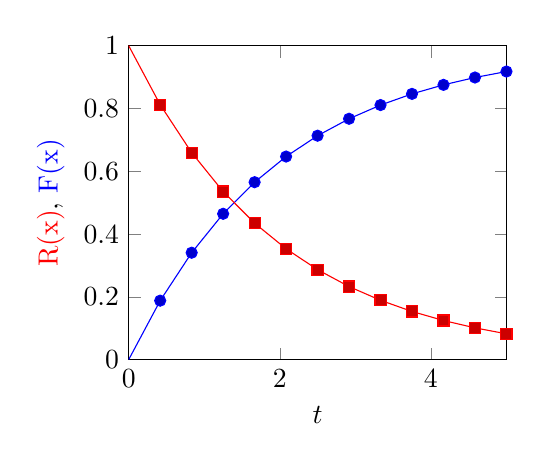
\begin{tikzpicture}
					\begin{axis}[ 
					xlabel=$t$,
					ylabel={\color{red}{R(x)}\color{black}, \color{blue}{F(x)}},
					ymin=0,
					xmin=0,
					ymax=1,
					xmax=5,
					scale=0.7,
					] 
					\addplot {1 - (e^(-0.5 * x))}; 
					\addplot {e^(-0.5 * x)}; 
					\end{axis}
			\end{tikzpicture}
			
			\end{multicols}
			
			\begin{align*}
				MTTF = \int\limits_{0}^\infty (1-F(t)) dt = \int\limits_{0}^\infty (e^{-\lambda t}) dt = \frac{1}{\lambda}					
			\end{align*}
			
			\underline{Reihenschaltung:}
			\begin{align*}
				R_{ges}(t)=\prod\limits_{i=1}^nR_i(t)=e^{-\lambda t} \text{ mit } \lambda=\sum\limits_{n=1}^n\lambda_i
			\end{align*}
			
			\underline{Parallelschaltung:}
			\begin{align*}
				F_{ges}(t)=\prod\limits_{i=1}^nF_i(t) \text{ also } R_{ges}(t)=1-\prod\limits_{i=1}^n(1-R_i(t))
			\end{align*}
			
			\underline{Mehrheitsentscheidung bei Redundanz durch mehrere Komponenten:}
			\begin{align*}
				R_{ges}=\sum\limits_{i=k}^n\binom{n}{i}R(t)^i(1-R(t))^{n-i}
			\end{align*}
			
	\chapter{Testen}
		\textbf{Verifikation:} Formaler Nachweis von Korrektheit und Einhalten der Spezifikation.\\
		\textbf{Testen:} Ausführen verschiedener Testfälle und Überprüfung des Ergebnisses. Vollständigkeit nahezu nie erreichbar.
		
		\section{Bugs}
			\begin{itemize}
				\item \textbf{Bohrbug:} Reproduzierbar; tritt immer unter den gleichen Umständen auf.
				\item \textbf{Heisenbug:} Tritt beim Versuch den Fehler zu analysieren nicht mehr auf.
				\item \textbf{Schrödinbug:} Wirkt sich nicht auf die Ausführung aus und lässt sich nur durch Codeanalyse finden.
			\end{itemize}
			
		\section{Testen}
			Extremfälle und ungültige Eingaben sollten immer auch getestet werden (vor allem bei Black Box).\\Beim White Box-Testing gibt es Statement/Line Coverage, Branch Coverage, Path Coverage, Multicondition/Predicate Coverage und Loop Coverage (jede Schleife mind. zwei mal).
		
		\section{Verifikation}
		Man kann den Code als endlichen Automaten abstrahieren (Kirpke-Struktur).\\
		Es gibt folgende Quantoren [Computation Tree Logic: CTL] (A,E Pfadquantoren; Rest Zustandsquantoren):
		\begin{itemize}
			\item[A] für jeden Pfad
			\item[E] es gibt einen Pfad
			\item[Xp] im nächsten Zustand gilt
			\item[Fp] irgendwann in der Zukunft gilt
			\item[Gp] es gilt in Zukunft immer
			\item[pUq] es gilt $p$ bis $q$ gilt
		\end{itemize}
